\documentclass{article}
\usepackage[pdftex]{graphicx}
%\usepackage[latin1]{inputenc}
\usepackage[utf8]{inputenc}

%Bordas da página
\usepackage{setspace}
\usepackage[inner=30mm,outer=20mm,top=30mm,bottom=20mm]{geometry}

%Fonte arial
\renewcommand{\rmdefault}{phv}

%layout
\pdfpagewidth 210mm
\pdfpageheight 297mm
%\inglespacing
\onehalfspacing
%\doublespacing
%\topmargin 0in
%\headheight 0in
%\headsep 0in
%\textheight 9in
%\textwidth 6.5in
%\oddsidemargin 0in
%\evensidemargin 0in

%To use \toprule, ...
\usepackage{booktabs}

\usepackage{multirow}

\usepackage{color}

\title{Simulação de Moduladores (AM DSB e DSB-SC) e Demodulador}

\author{Pedro Batista (08080002701) pedro@ufpa.br}

\begin{document}

\maketitle

\section{Modulador e Demodulador AM DSB}
O modulador simulado é representado pela equação~\ref{eq:dsb}. A configuração
adotada é mostrada na Figura~\ref{fig:dsb_conf}. No demodulador temos um filtro
passa baixas, com frequência de corte $f_c$. O modelo criado no \texttt{Simulink}
é mostrado na Figura~\ref{fig:dsb_model} e os sinais resultantes são mostrados na
Figura~\ref{fig:dsb_result}.
\begin{equation}\label{eq:dsb}
s(t)=A_c[1+k_am(t)]cos(2\pi f_ct)
\end{equation}
\begin{figure}[h]
\begin{equation}
m(t)=\sin(2\pi f_st)
\end{equation}
\begin{equation}
A_c=1
\end{equation}
\begin{equation}
k_a=0.5
\end{equation}
\begin{equation}
f_c=100
\end{equation}
\begin{equation}
f_s=10
\end{equation}
\caption{Configuração adotada na simulação DSB.}
\label{fig:dsb_conf}
\end{figure}

\begin{figure}[h]
   \centering
   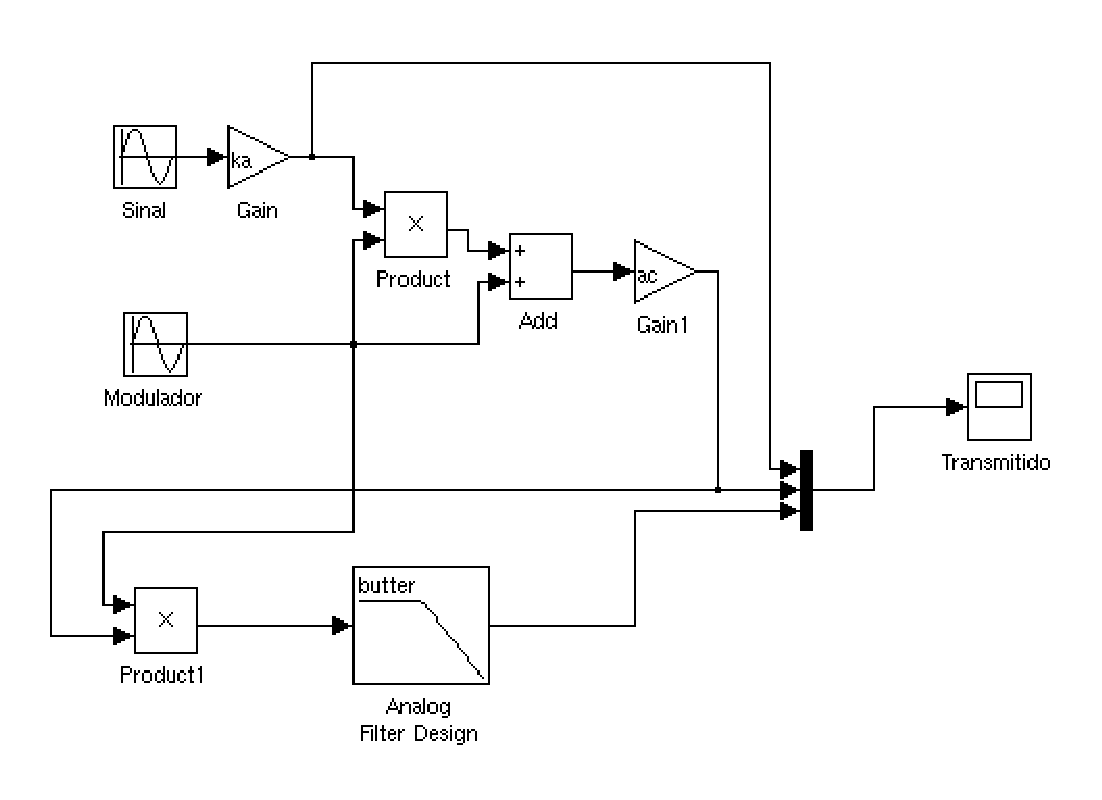
\includegraphics[height=5cm]{dsb_model}
   \caption{Modelo no Simulink para transmissor e receptor AM DSB.}
   \label{fig:dsb_model}
\end{figure}
\begin{figure}[h]
   \centering
   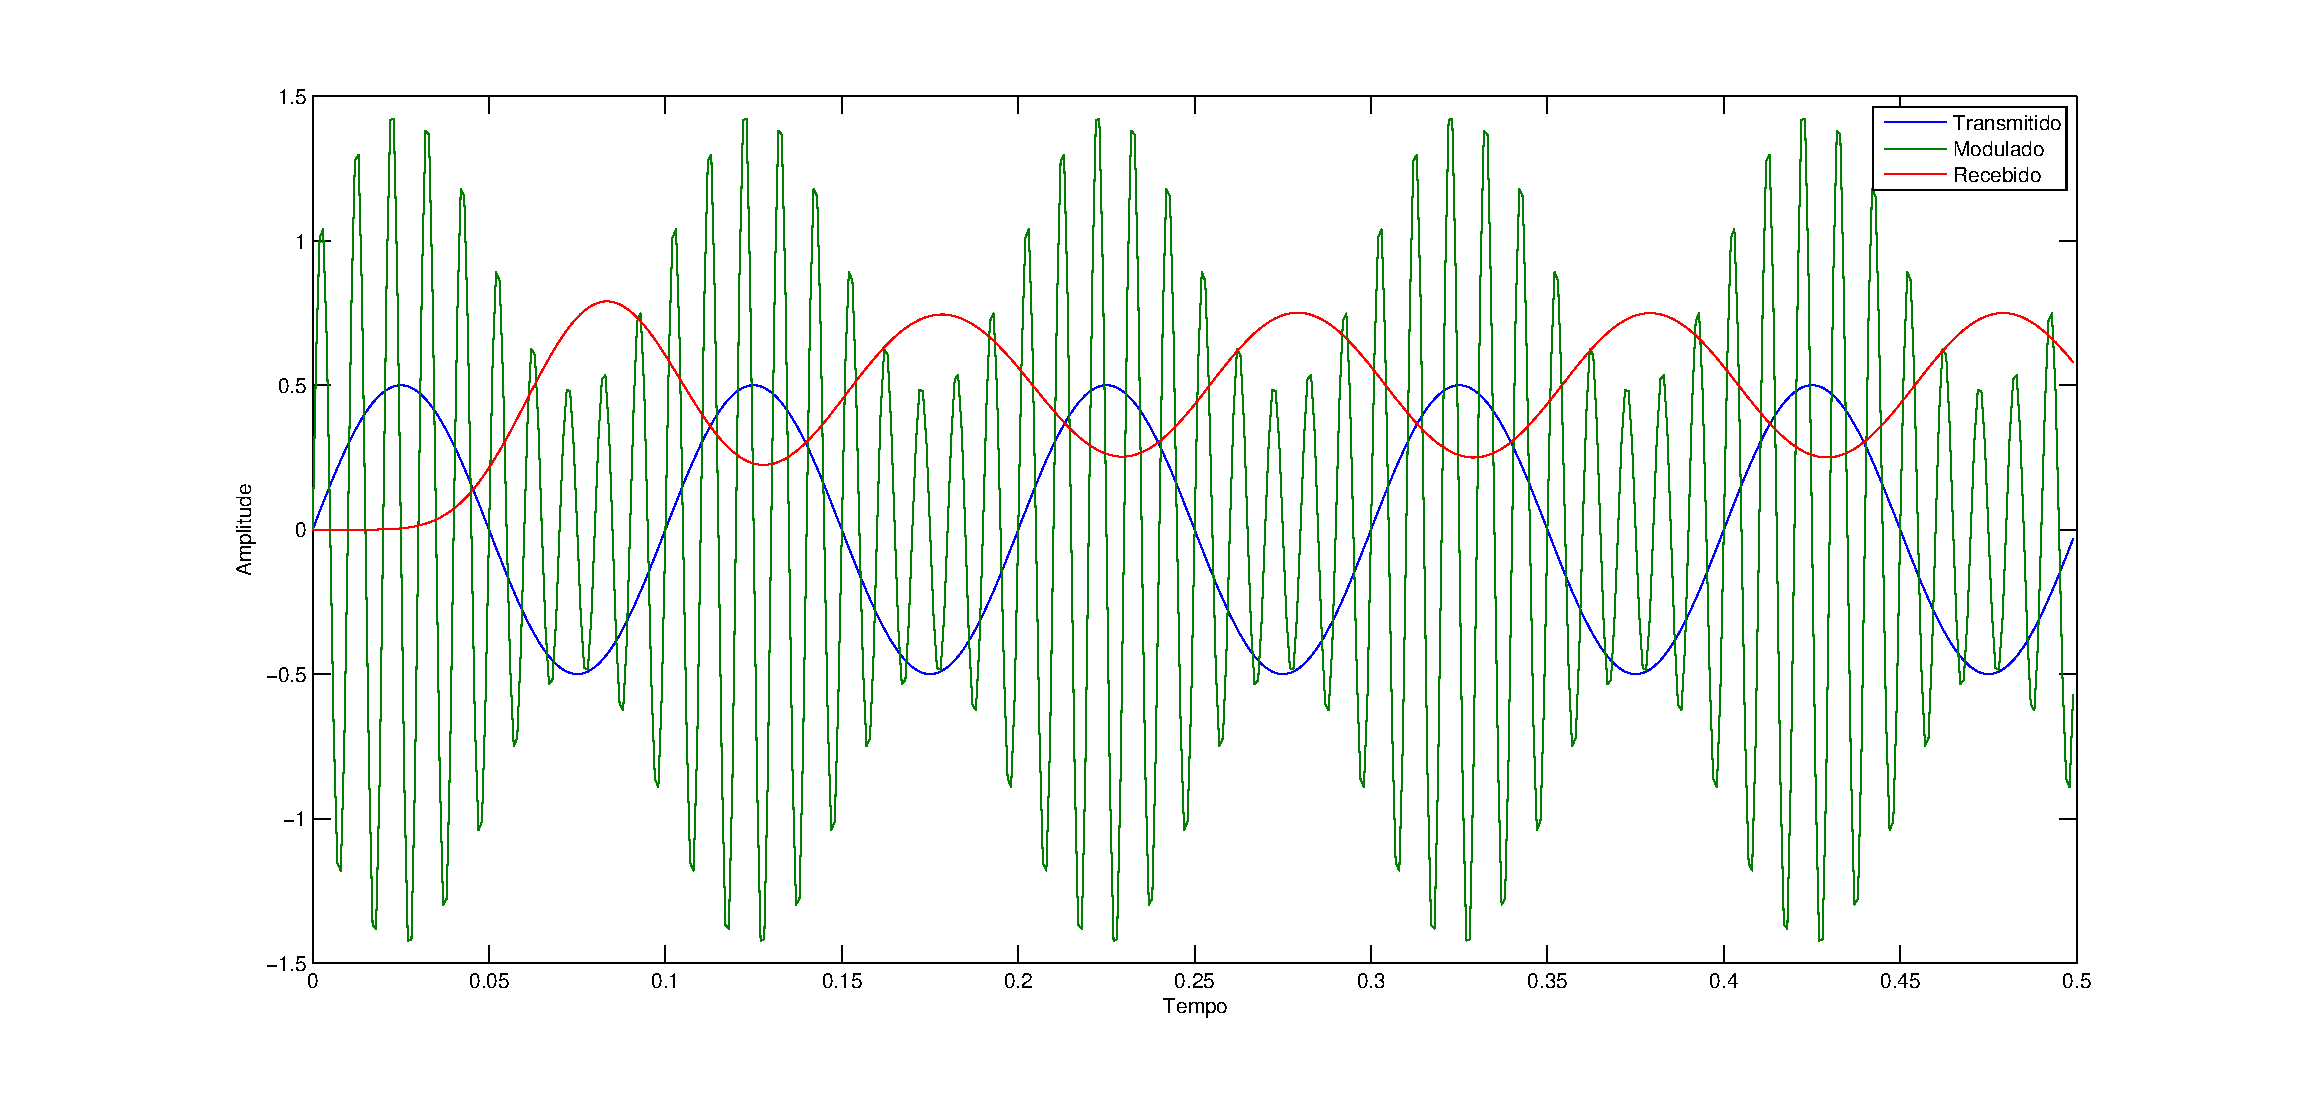
\includegraphics[height=8cm]{dsb_result}
   \caption{Sinais resultantes da simulação de transmissor e receptor AM DSB.}
   \label{fig:dsb_result}
\end{figure}

\section{Modulador e Demodulador AM DSB-SC}
Para o modulador AM DSB-SC dado pela equação~\ref{eq:dsb-sc}, foram utilizadas as configurações
mostradas na Figura~\ref{fig:dsb-sc_conf}. O demodulador possui um filtro passa baixas, com 
frequência de corte igual a $f_c$. O modelo criado no \texttt{Simulink} é mostrado na
Figura~\ref{fig:dsb-sc_model}, e os sinais resultantes na Figura~\ref{fig:dsb-sc_result}.

\begin{equation}\label{eq:dsb-sc}
s(t)=A_cm(t)\cos(2\pi f_ct)
\end{equation}

\begin{figure}[h]
\centering
\begin{equation}
m(t)=\sin(2\pi f_st)
\end{equation}
\begin{equation}
A_c=1
\end{equation}
\begin{equation}
f_c=100
\end{equation}
\begin{equation}
f_s=10
\end{equation}
\caption{Configuração adotada na simulação DSB-SC.}
\label{fig:dsb-sc_conf}
\end{figure}

\begin{figure}[h]
   \centering
   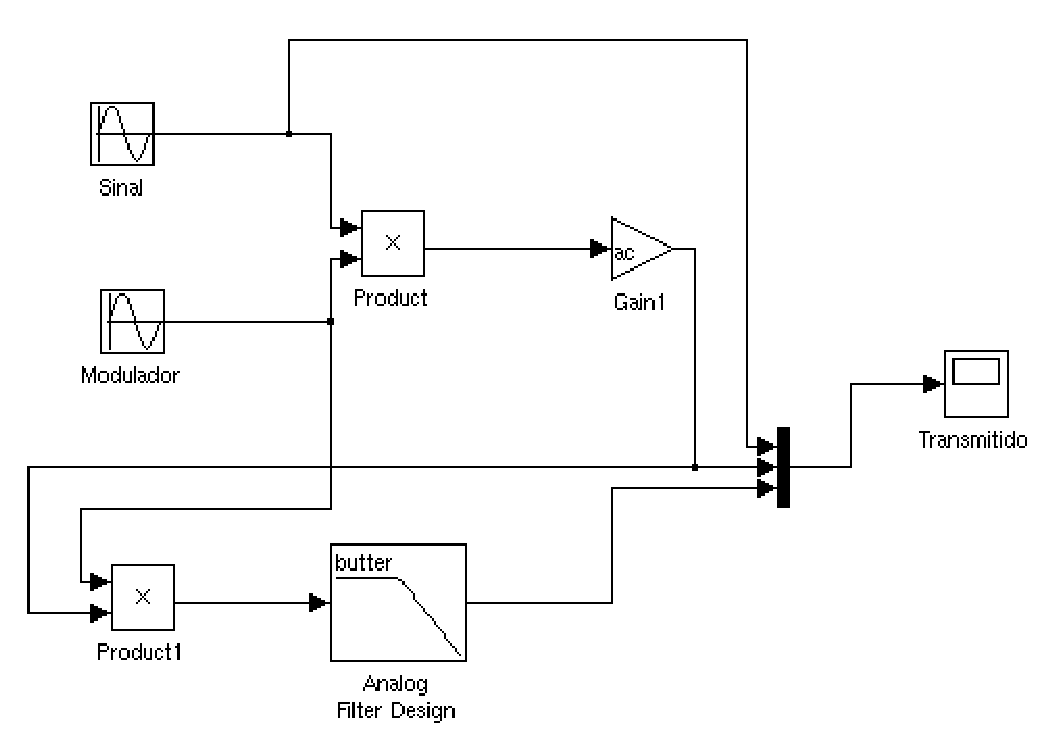
\includegraphics[height=5cm]{dsb-sc_model}
   \caption{Modelo no Simulink para transmissor e receptor AM DSB-SC.}
   \label{fig:dsb-sc_model}
\end{figure}
\begin{figure}[h]
   \centering
   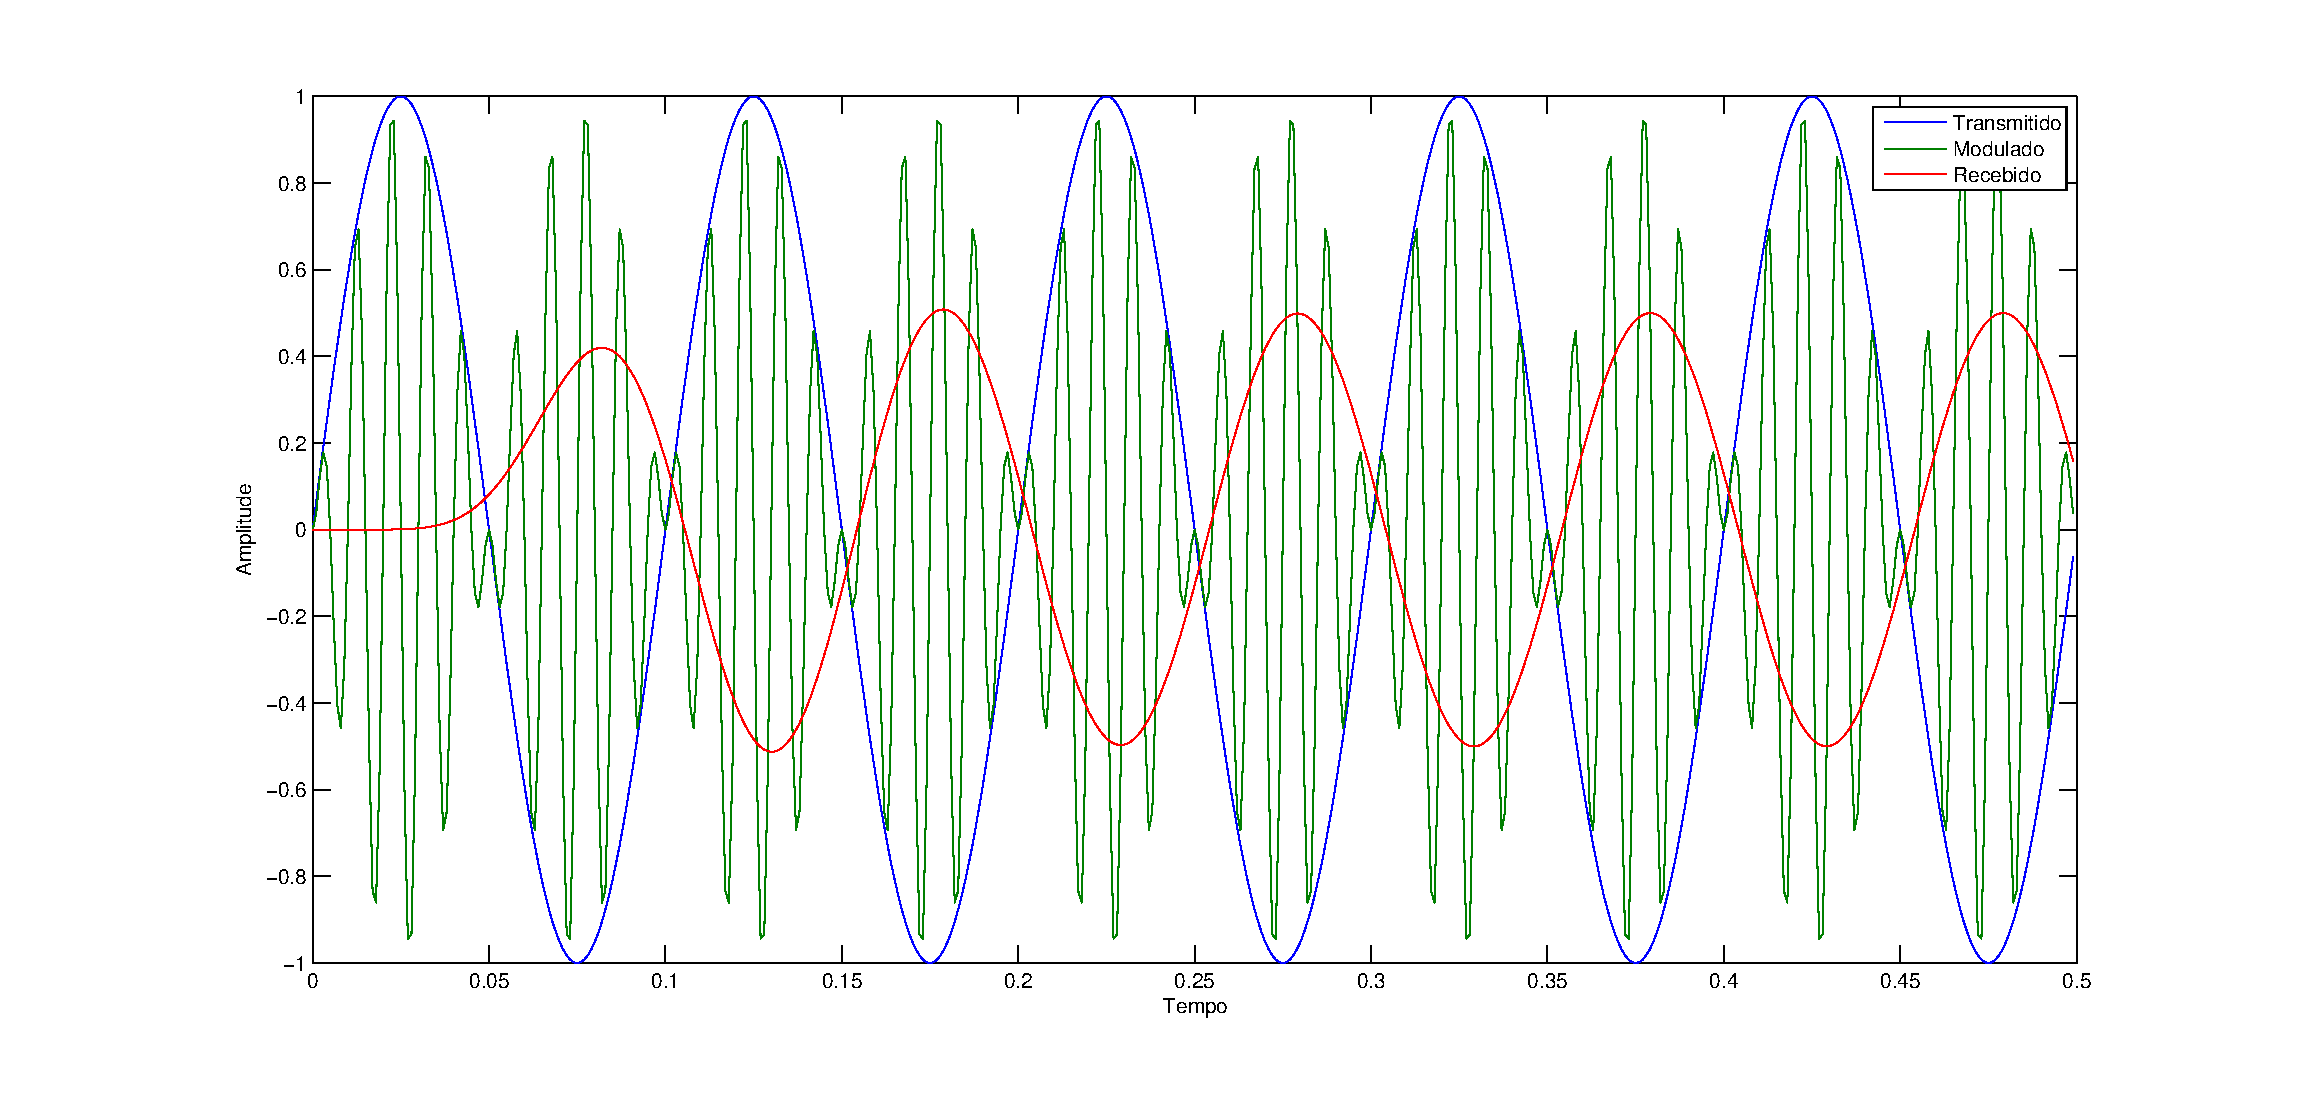
\includegraphics[height=8cm]{dsb-sc_result}
   \caption{Sinais resultantes da simulação de transmissor e receptor AM DSB-SC.}
   \label{fig:dsb-sc_result}
\end{figure}

\bibliographystyle{plain}
\bibliography{bib}

\end{document}
